%auto-ignore
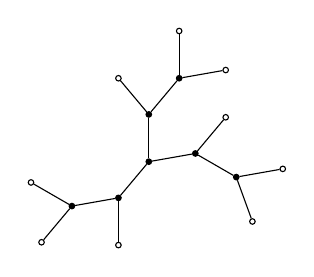
\begin{tikzpicture}

\def\rad{1cm}
\def\angdist{140}
\def\posa{90}
\def\extlen{0.6cm}

\tikzset{point/.style = {draw, circle, fill=black, minimum size=2pt,inner sep=0pt}}


\coordinate[point] (C1) at (0,0) {};
\path (C1) node[point] (C11)  at +(\posa:\extlen) {};
\path (C1) node[point] (C12)  at +(\posa+\angdist:\extlen) {};
\path (C1) node[point] (C13)  at +(\posa+2*\angdist:\extlen) {};
\draw (C1) -- (C11);
\draw (C1) -- (C12);
\draw (C1) -- (C13);

\path (C11) node[point] (C111)  at +(-180+\posa+\angdist:\extlen) {};
\path (C11) node[point,style={fill=white}] (C112)  at +(-180+\posa-\angdist:\extlen) {};
\draw (C11) -- (C111);
\draw (C11) -- (C112);

\path (C12) node[point] (C121)  at +(-180+\posa+\angdist + \angdist:\extlen) {};
\path (C12) node[point,style={fill=white}] (C122)  at +(-180+\posa+\angdist - \angdist:\extlen) {};
\draw (C12) -- (C121);
\draw (C12) -- (C122);

\path (C13) node[point] (C131)  at +(-180+\posa+2*\angdist + \angdist:\extlen) {};
\path (C13) node[point,style={fill=white}] (C132)  at +(-180+\posa+2*\angdist - \angdist:\extlen) {};
\draw (C13) -- (C131);
\draw (C13) -- (C132);


\path (C121) node[point,style={fill=white}] (C1211)  at +(-180-180+\posa+\angdist + \angdist+\angdist:\extlen) {};
\path (C121) node[point,style={fill=white}] (C1212)  at +(-180-180+\posa+\angdist + \angdist-\angdist:\extlen) {};
\draw (C121) -- (C1211);
\draw (C121) -- (C1212);

\path (C111) node[point,style={fill=white}] (C1112)  at +(-180-180+\posa+\angdist+\angdist:\extlen) {};
\path (C111) node[point,style={fill=white}] (C1111)  at +(-180-180+\posa+\angdist-\angdist:\extlen) {};
\draw (C111) -- (C1111);
\draw (C111) -- (C1112);

\path (C131) node[point,style={fill=white}] (C1312)  at +(-180-180+\posa+2*\angdist + \angdist+\angdist:\extlen) {};
\path (C131) node[point,style={fill=white}] (C1311)  at +(-180-180+\posa+2*\angdist + \angdist-\angdist:\extlen) {};
\draw (C131) -- (C1311);
\draw (C131) -- (C1312);

\end{tikzpicture}